%\usetikzlibrary{decorations.pathmorphing,patterns}

\chapter{Dynamics}
\label{chapter:dynamics}

%\section[Intro]{Introduction}

Now that we can mathematically describe the motion of any object, we have to
be able describe \emph{what} causes motion, or more precisely,
\emph{what causes motion to change.}




\section{Laws of Motions}
The definitions given here are based on the original text by Newton in
\emph{Principia}, but with some wording replaced with modern physics
language\footnote{For example, Newton used the term \emph{the alteration of
motion} to describe the acceleration of the object.}

The first law of motion describes what happens when there are no forces act on
an object:
\begin{definition}
  \textbf{First law:} Every object remains at rest or in uniform motion, until
  there is a net external force acting on the object.
\end{definition}
In other words, when the vector sum of all the forces acting on an object is
zero, the object's velocity does not change. In other words, the three equations
below are equivalent:
\begin{equation*}
  \bm F_\text{net}=\sum\bm F=\bm 0
  \quad\longleftrightarrow\quad
  \bm v=\text{constant}
  \quad\longleftrightarrow\quad
  \bm a=\bm 0
\end{equation*}
%  \end{center}
%  \begin{itemize}
%  \item As long as an object moves in uniform motion, it must be that
%    $\bm F_\text{net}=\bm 0$
%  \item Examples:
%    \begin{itemize}
%    \item A spacecraft in ``deep space'' has no forces acting on it
%    \item A hockey puck sliding on very smooth ice has gravity and normal
%      force, but the net force is zero
%    \item A car travelling on a highway at \SI{100}{\kilo\metre\per\hour} has
%      many forces acting on it, but the net force is zero
%    \end{itemize}
%  \item In ``a state of equilibrium''
%  \end{itemize}

What is not stated explicitly by Newton is that the first law of motion is only
valid when the mass of the object is constant. In other words, the first law of
motion, as stated above, will \emph{not} work for:
\begin{itemize}[itemsep=3pt]
\item A rocket expelling spent fuel as it is launched towards space
\item A train car collecting grain though its open top
\end{itemize}
Later in Chapter~\ref{chapter:momentum}, we will modify the first law of motion
to include objects with changing mass.


The secon law of motion addresses what happens when the forces acting on an
object is not balance, i.e.\ when the net force is not zero.

\begin{definition}
  \textbf{Second law:} The acceleration of an object is proportional to the
  sum of all forces (net force) acting on it; and is along the same
  direction as the net force.
\end{definition}
The second law states that the acceleration of an object is the direct result
of the imbalance of forces, and that the relationship is \emph{linear} (i.e.\
when the net force is double, the acceleration also doubles). The first two
laws of motion can be summarized by perhaps one of the most important and
recognizable equations in physics:
\begin{equation}
  \boxed{\bm F_\text{net}=m\bm a}
\end{equation}
The \emph{proportionality} between the net force and the acceleration of the
object is its mass. In fact, mass is defined as the ratio between the magnitude
of the net force acting on an object and the magnitude of the resultant
acceleration:
\begin{equation}
  m=\frac{|\bm F_\text{net}|}{|\bm a|}
\end{equation}
As such, mass is an intrinsic property of an object, and the same net force on
the object will \emph{always} result in the same acceleration, regardless of
what the net force is composed of, and whether the object is on Earth, on the
Moon, or in deep space.

Both the first and second laws of moton, as stated by Newton, require that the
mass of the object be constant. 




The third law of motion deals with the interaction between objects when forces
are created, and how objects apply forces on each other:
\begin{definition}
  \textbf{Third Law:} To every action there is always opposed and equal
  reaction; the mutual actions of two bodies upon each other are always
  equal, and directed to contrary parts.
\end{definition}
Mathematically, we can write that the force object $A$  exerts on bbject $B$
($\bm F_{AB}$, the action force) is equal in magnitude but opposite in
direction to the force that object $B$ exerts on object $A$ ($\bm F_{BA}$, the
reaction force).
\begin{equation}
  \boxed{\bm F_\text{AB} = -\bm F_\text{BA}}
  \label{eq:third-law}
\end{equation}
The negative sign in Eq.~\ref{eq:third-law} indicates that the forces are in
opposite direction. It must be noted that
\textbf{the action and reaction forces must act on \emph{different} objects}.

The implication of the laws of motion is that forces are always created in
pairs: it is impossible for one object to exert a force on another without also
simultaneously being acted on by the other object. In
Chapter~\ref{chapter:energy}, we will show that the third law of motion is
crucial in formulating, and understanding, the law of conservation of energy.
In Chapter~\ref{chapter:momentum}, we will show that the third law of motion
is, in fact, an application of the first law of motion.

%\begin{example}
%  Old-style television picture tubes and computer monitors use cathode ray
%  tubes, where light is produced when fast-moving electrons collide with
%  phosphor molecules on the surface of the screen. The electrons (mass
%  $m=\text{\SI{9.1e-31}{\kilo\gram}}$) are accelerated from rest in the
%  electron ``gun'' at the back of the vacuum tube. Find the velocity of an
%  electron when it exits the gun after experiencing an electric force of
%  \SI{5.8e-15}{\newton} over a distance of \SI{3.5}{\milli\metre}.
%\end{example}

\section{Common Forces}
%  \textbf{Force} is the interaction between the objects
%  \begin{itemize}
%  \item When there is interaction, then forces are created
%  \item A ``push'' or a ``pull''
%  \end{itemize}
%
%  \vspace{.2in}There are two types of forces:
%  \begin{itemize}
%  \item\textbf{Contact forces} act between two objects that are in contact
%    with one another
%  \item\textbf{Non-contact forces} act between two objects without them
%    touching each other.
%    \begin{itemize}
%    \item Also called ``action-at-a-distance'' force
%    \end{itemize}
%  \end{itemize}
%
%
%
%
%\section{Forces}
%  Newton considered all forces acting at a single point of an object called the
%  centre of mass (``CM'')
%  \begin{itemize}
%  \item The centre of mass is also called the centre of gravity (``CG'') if the
%    object is inside a uniform gravitational field\footnote{Gravitational field
%    is a topic that will be discussed in Class 7}
%  \item If the density of an object is constant, then the CM is also the
%    geometric centre (centroid) of the object
%  \end{itemize}
%%  \vspace{.2in}If the net force on an object is zero ($\sum\bm F=\bm{0}$)
%%  then the object is in a \emph{state of equilibrium}
%%  \begin{itemize}
%%  \item Dynamic equilibrium: the object is moving relative to us
%%  \item Static equilibrium: the object is not moving relative to us
%%  \end{itemize}




\begin{itemize}[noitemsep]
\item Gravitational force ($\bm F_g$)
\item Normal force ($\bm F_n$)
\item Static and kinetic friction ($\bm F_s$ and  $\bm F_k$)
\item Spring force ($\bm F_e$)
\item Tension ($\bm F_T$)
\item Fluid Resistance, or Drag ($\bm F_d$)
\item Applied force ($\bm F_a$)
\item Electrostatic force ($\bm F_q$, discussed in Unit 3)
\item Magnetic force ($\bm F_m$, discussed in Unit 3)
\end{itemize}




\subsection{Gravity}
\textbf{Gravity} is the mutual force of attraction between all massive objects.
The gravitational force that objects apply to each other can be expressed as:
\begin{equation}
  \boxed{\bm F_g=m\bm g}
\end{equation}
The gravitational force acts in the same direction as $\bm g$, the acceleration
due to gravity at the object's position. At or near the surface of Earth,
$\bm g=\text{\SI{9.81}{\metre\per\second\squared}}$ [down]. In fact, the
direction of $\bm g$ is how we \emph{define} the concept of ``down''. $\bm g$
is also known as the ``gravitational field''; will be discussed in depth in
Chapter~\ref{chapter:gravity}. If this is the only force that acts on an object,
its resulting motion is called \textbf{free fall}.

To be clear, by the third law of motion, any object that is subjected to the
gravitational pulled by Earth will also exert an equal and opposite force on
Earth. However, since Earth is much more massive, this force will have no
effect to Earth's motion.

\subsection{Normal Force}
\textbf{Normal force} $F_n$ is a force a surface exerts on another object
that it is in contact with. It is always \emph{perpendicular} to the contact
surface.\footnote{This is where the term \emph{normal} came from.}

\begin{figure}[ht]
  \centering
  \begin{tikzpicture}
    \draw[thick] (-1,0)--(2.5,0);
    \draw[mass] rectangle (1.5,1);
    \fill (.75,.5) circle (2pt);
    \draw[vectors] (.75,.5)--+(0,-1) node[below]{$F_g$};
    \draw[vectors] (.75,.5)--+(0,1) node[above]{$F_n$};
  \end{tikzpicture}
  \hspace{.5in}
  \begin{tikzpicture}
    \begin{scope}[rotate=30]
      \draw[thick] (-1,0)--(2.5,0);
      \draw[mass] rectangle (1.5,1);
      \fill (.75,.5) circle (2pt);
      \begin{scope}[vectors]
        \draw[rotate around={-30:(.75,.5)}] (.75,.5)--+(0,-1)
        node[below]{$F_g$};
        \draw (.75,.5)--+(0,1) node[above]{$F_n$};
      \end{scope}
    \end{scope}
  \end{tikzpicture}
\end{figure}
Regardless of whether the surface is horizontal or slanted, $F_n$ is always be
perpendicular to the surface. However, the \emph{magnitude} of the normal force
will change.




%%\section{Normal Force on an Incline}
%%  When an object sits on a stationary incline, normal force decreases.
%%  
%%    \centering
%%    \begin{tikzpicture}[scale=.9]
%%      \draw[thick] (-1,0)--(3,0);
%%      \draw[thick,->] (0,0) arc (0:37:1) node[midway,right] {$\theta$};
%%      \begin{scope}[rotate around={37:(-1,0)}]
%%        \draw[->](3.5,.5)--(4,.5)  node[right]{$x$};
%%        \draw[->](3.5,.5)--(3.5,1) node[above]{$y$};
%%        \draw[thick] (-1,0)--(4,0);
%%        \draw[fill=pink,thick] rectangle (3,2);
%%        \fill(1.5,1) circle (.07) node[right]{CM};
%%        \begin{scope}[->,thick,red]
%%          \draw[dotted] (1.5,1)--(1.5,-.5) node[right]{$F_g\cos\theta$};
%%          \draw[dotted] (1.5,1)--(.45,1) node[left]{$F_g\sin\theta$};
%%        \end{scope}
%%        \draw[->,very thick,red] (1.5,1)--(.45,-.5)
%%        node[below]{$F_g$}
%%        node[pos=.3,below right]{$\theta$};
%%        \draw[->,very thick] (1.5,1)--(1.5,2.5) node[above]{$F_n$};
%%      \end{scope}
%%    \end{tikzpicture}
%%    
%%    \begin{itemize}
%%    \item $F_n=F_g\cos\theta$
%%    \item $F_g$ has a component along the ramp $F_g\sin\theta$ that
%%      wants to slide the block down.
%%    \item There may also be a friction force $F_f$ that opposes the motion
%%    \item If the incline is also accelerating, then we have to treat this
%%      problem as a connected-body problem (discussed later in this topic)
%%    \end{itemize}

\subsection{Friction}
\textbf{Friction} is force that opposes the sliding of two surface across one
another
\begin{itemize}
\item Always act in the direction opposite to motion or attempted motion
\item Two types: \emph{static friction} and \emph{kinetic friction}
\end{itemize}  
%  \begin{center}
%   \pic{.6}{graphics/friction}
%  \end{center}


\textbf{Static friction} is the resistive force between two surfaces when
there is no relative motion between them. It increases with increasing
applied force $F_a$. It is at maximum when the object is just about to move.
\begin{equation}
  \boxed{
    F_s \leq \mu_sF_n
  }
  \label{eq:static-friction}
\end{equation}
\begin{center}
  \begin{tabular}{l|c|c}
    \rowcolor{pink}
    \textbf{Quantity} & \textbf{Symbol} & \textbf{SI Unit} \\ \hline
    Magnitude of static friction   & $F_s$ & \si\newton \\
    Coefficient of static friction & $\mu_s$ & (no unit)\\
    Magnitude of normal force      & $F_n$ & \si\newton
  \end{tabular}
\end{center}
Equation~\ref{eq:static-friction} only deals with the \emph{magnitude} of the
force. A proper free-body diagram is required to express the direction of
$\bm F_s$
%  \begin{tikzpicture}[overlay]
%    \uncover<2>{
%      \node[text width=85,draw=violet,fill=violet!5,text=violet] (act) at
%      (-3.2,4) {Actual static friction};
%      \draw[axes,violet] (act)--+(3,0);
%      
%      \node[text width=100,draw=orange,fill=orange!5,text=orange] (max) at
%      (5.05,4) {Maximum static friction};
%      \draw[axes,orange] (max)--+(-3,0);
%    }
%  \end{tikzpicture}

\textbf{Kinetic friction} is the resistive force between two surfaces that
are moving relative to each other. It is (nearly) constant along the path of
movement as long as the normal force stays constant:
\begin{equation}  
  \boxed{F_k = \mu_kF_n}
\end{equation}
\begin{center}
  \begin{tabular}{l|c|c}
    \rowcolor{pink}
    \textbf{Quantity} & \textbf{Symbol} & \textbf{SI Unit} \\ \hline
    Magnitude of kinetic friction   & $F_k$   & \si{\newton}\\
    Coefficient of kinetic friction & $\mu_k$ & (no unit)\\
    Magnitude of normal force       & $F_n$   & \si{\newton}
  \end{tabular}
\end{center}    
$\mu_k$ is always lower than $\mu_s$, otherwise nothing will ever move:
\begin{equation}  
  \mu_k\leq\mu_s
\end{equation}

%  \begin{tikzpicture}[overlay]
%    \uncover<2>{
%      \node[text width=86,draw=magenta,fill=magenta!5,text=magenta] (act) at
%      (3.5,5) {Unlike static friction, this is an equality};
%      \draw[axes,magenta] (act) to[out=50,in=90] +(3.5,.25);
%    }
%  \end{tikzpicture}




\subsection{Tension in a Cable}
\textbf{Tension} is the force exerted on and by a cable, rope, or string.
\begin{itemize}
\item You can't push on a rope
\item Assume the cable/rope/string to be mass less
\item Force can change direction when used with pulleys
\end{itemize}
How do engineers determine the amount of tension needed for a specific object
(bridges, floors or light fixtures)?




\subsection{Spring Force}
The spring force $\bm F_e$ is the force that a compressed/stretched spring
exerts on the object connected to it. An \emph{ideal} spring obeys
\textbf{Hooke's law}:
\begin{equation}
  \boxed{
    \bm F_e=-k\bm x
  }
\end{equation}
$\bm F_e$ is in the opposite direction to the spring's displacement $\bm x$,
and is proportional to the amount of compression/stretching.

\begin{center}
  \begin{tikzpicture}[scale=.8]
    \draw[mass] (5,.5) rectangle (6,1.5);
    \draw[thick,
      decoration={aspect=.6,segment length=5mm, amplitude=2.5mm, coil},
      decorate] (0,1)--(5,1);
    \fill[pattern=north east lines](-.2,0) rectangle (0,2);
    \draw[thick] (0,0)--(0,2);
    \fill[red] (5.5,1) circle (.06);
    \draw[vectors,red] (5.5,1)--(4,1) node[above]{$\bm F_e$};
    \draw[dashed] (3,0)--(3,2) node[above]{Equilibrium position};
    \draw[vectors] (3,.3)--(5,.3) node[midway,below]{$x$};
  \end{tikzpicture}
  \hspace{.2in}
  \begin{tikzpicture}[scale=.8]
    \draw[thick,gray!40,fill=gray!20] (5,.5) rectangle (6,1.5);
    \draw[thick,gray!20,
      decoration={aspect=.6,segment length=5mm, amplitude=2.5mm, coil},
      decorate] (0,1)--(5,1);
    \fill[pattern=north east lines] (-.2,0) rectangle(0,2);
    \draw[thick] (0,0)--(0,2);
    \fill[gray!30] (5.5,1) circle (.06);
    \draw[vectors,gray!30] (5.5,1)--(4,1) node[above]{$\bm F_e$};
    \draw[dashed] (3,0)--(3,2);
    \draw[vectors,gray!30] (3,.3)--(5,.3) node[midway,below]{$x$};
    \draw[mass] (1.5,.5) rectangle (2.5,1.5);
    \draw[thick,
      decoration={aspect=.3,segment length=1.5mm, amplitude=2.5mm, coil},
      decorate] (0,1)--(1.5,1);
    \draw[vectors] (3,.3)--(1.5,.3) node[midway,below]{$x$};
    \fill[red] (2,1) circle (.06);
    \draw[vectors,red] (2,1)--(3,1) node[above]{$\bm F_e$};
  \end{tikzpicture}
\end{center}
The constant $k$ (called the \textbf{spring constant}, \textbf{force
  constant}, \textbf{Hooke's constant} or \textbf{spring rate}) is the
stiffness of the spring. It has a unit of \si{\newton\per\metre}.



\subsection{Fluid Resistance (Drag)}

When an object (e.g.\ an aircraft, a bicycle or a car) moves through air, or
when a submarine moves under water, they all experience a
fluid\footnote{A gas or a liquid} resistance force called the
\textbf{drag} $\bm F_d$.
\begin{figure}[ht]
  \centering
  \begin{subfigure}{.338\textwidth}
    \pic1{dynamics/boeing787}
    \caption{A commercial aircraft flying through air}
  \end{subfigure}
  \begin{subfigure}{.35\textwidth}
    \pic1{dynamics/ganna}
    \caption{A cyclist riding at high speed during a bike race}
  \end{subfigure}
  \begin{subfigure}{.263\textwidth}
    \pic1{dynamics/submarine}
    \caption{A submarine moving through water}
  \end{subfigure}
\end{figure}
The drag force is experienced by any object moving through a fluid. The
direction of drag is in the opposite direction to the velocity vector.

There are multiple sources of drag:
\begin{itemize}
\item\textbf{form drag} is due to the shape of the object
\item\textbf{skin friction} is due to the friction of the fluid against
  the surface of the object moving through it
\item\textbf{interference drag} is due to when airflow around one part of
  an object occupying the same space as the airflow around another part
  (e.g.\ fuselage and wing of an airplane)
\end{itemize}

Unlike kinetic friction (which is constant), drag depend on the speed of the
moving object, as well as its shape:
\begin{equation}
  \boxed{
    F_d=\frac12\rho v_\infty^2C_DA_\text{ref}
  }
\end{equation}
\begin{center}
  \begin{tabular}{l|c|c}
    \rowcolor{pink}
    \textbf{Quantity} & \textbf{Symbol} & \textbf{SI Unit} \\ \hline
    Magnitude of drag       & $F_d$     & \si\newton \\
    Density of the fluid    & $\rho$    & \si{\kilo\gram\per\metre\cubed}\\
    Free-stream velocity    & $v_\infty$ & \si{\metre\per\second} \\
    Reference area          & $A_\text{ref}$ & \si{\metre\squared} \\
    Drag coefficient        & $C_D$     & (no unit)
  \end{tabular}
\end{center}
$C_D$ depends on the shape and surface smoothness of the object; for bluff
bodies $A_\text{ref}$ is the frontal area; for streamlined objects
$A_\text{ref}$ is the planform (top-view) area




\section{Free Body Diagrams}
A free-body diagram is used to visualize the forces acting on an object. It is
very useful tool that should be used all the time.
\emph{We generally draw the forces from an inertial frame of reference.}

\begin{enumerate}
\item Draw a ``big dot'' to represent the centre of mass of the object.
%  \vspace{.1in}
%  
%    \centering
%    \begin{tikzpicture}[scale=.8]
%      \draw[lightgray,thick] (-1,0)--(4,0);
%      \draw[lightgray,fill=cyan!10,thick] rectangle (3,2);
%      \fill (1.5,1) circle (.1) node[above]{CM};
%    \end{tikzpicture}
%    
%    \centering
%    \begin{tikzpicture}[scale=.8]
%      \begin{scope}[rotate=30]
%        \draw[lightgray,thick] (0,0)--(5,0);
%        \draw[lightgray,fill=cyan!10,thick] (1,0) rectangle (4,2);
%        \fill (2.5,1) circle (.1) node[above]{CM};
%      \end{scope}
%      \draw[lightgray,thick] (0,0)--(4.5,0);
%    \end{tikzpicture}
%    
%    \centering
%    \begin{tikzpicture}[scale=.8]
%      \draw[lightgray,fill=cyan!10,thick] circle (.5);
%      \fill circle (.1) node[above]{CM};
%    \end{tikzpicture}
%  
%
%
%
%
%\section{Free Body Diagrams}
\item Define a coordinate system ($x$ and $y$ axes)
  \begin{itemize}
  \item Axes are defined to simplify the problem (not to make it more
    complicated!)
  \item Define coordinate system such that motion is along one axis (usually
    $x$) only
  \end{itemize}

%  \vspace{.1in}
%  
%    \centering
%    \begin{tikzpicture}[scale=.8]
%      \draw[lightgray,thick] (-1,0)--(4,0);
%      \draw[lightgray,fill=cyan!10,thick] rectangle (3,2);
%      \fill (1.5,1) circle (.1);
%      \draw[axes] (3.5,.5)--(4.5,.5) node[right]{$x$};
%      \draw[axes] (3.5,.5)--(3.5,1.5) node[above]{$y$};
%    \end{tikzpicture}
%    
%    \centering
%    \begin{tikzpicture}[scale=.8]
%      \begin{scope}[rotate=30]
%        \draw[lightgray,thick] (0,0)--(5,0);
%        \draw[lightgray,fill=cyan!10,thick] (1,0) rectangle (4,2);
%        \fill (2.5,1) circle (.1);
%        \draw[axes] (4.5,.5)--(5.5,.5)  node[right]{$x$};
%        \draw[axes] (4.5,.5)--(4.5,1.5) node[above]{$y$};
%      \end{scope}
%      \draw[lightgray,thick] (0,0)--(4.5,0);
%    \end{tikzpicture}
%    
%    \centering
%    \begin{tikzpicture}[scale=.8]
%      \draw[lightgray,fill=cyan!10,thick] circle (.5);
%      \fill circle (.1);
%      \draw[axes] (1,0)--(2,0) node[right]{$x$};
%      \draw[axes] (1,0)--(1,1) node[above]{$y$};
%    \end{tikzpicture}
%
%
%
%
%
%\section{Free Body Diagrams}
\item Identify and label all forces acting on the object
  \begin{itemize}
  \item If it has mass, weight $\bm F_g$ acts downward
  \item If it is on a surface, there is also a normal force $\bm F_n$
  \item If there is friction, first think about which direction the object will
    move without it, then draw $\bm F_s$ or $\bm F_k$ in the opposite
    direction
  \item If it is being pushed/pulled, there may be an applied force
    $\bm F_a$ or tension force $\bm F_T$
  \end{itemize}

%  
%    \centering
%    \begin{tikzpicture}[scale=.8]
%      \draw[lightgray,thick] (-1,0)--(4,0);
%      \draw[lightgray,fill=cyan!10,thick] rectangle (3,2);
%      \fill (1.5,1) circle (.1);
%      \draw[axes] (3.5,.5)--(4.5,.5) node[right]{$x$};
%      \draw[axes] (3.5,.5)--(3.5,1.5) node[above]{$y$};
%      \draw[vectors] (1.5,1)--(1.5,-.5) node[below]{$\bm F_g$};
%      \draw[vectors] (1.5,1)--(1.5,2.5) node[above]{$\bm F_n$};
%      \draw[vectors] (1.5,1)--(3.1,1) node[below]{$\bm F_a$};
%      \draw[vectors] (1.5,1)--(.75,1) node[left]{$\bm F_f$};
%    \end{tikzpicture}
%    
%    \centering
%    \begin{tikzpicture}[scale=.8]
%      \draw[lightgray,thick] (0,0)--(4.5,0);
%      \begin{scope}[rotate=30]
%        \draw[lightgray,thick] (0,0)--(5,0);
%        \draw[lightgray,fill=cyan!10,thick] (1,0) rectangle (4,2);
%        \fill (2.5,1) circle (.1);
%        \draw[axes] (4.5,.5)--+(1,0) node[right]{$x$};
%        \draw[axes] (4.5,.5)--+(0,1) node[above]{$y$};
%        \draw[vectors,rotate around={-30:(2.5,1)}] (2.5,1)--(2.5,-.5)
%        node[below]{$\bm F_g$};
%        \draw[vectors] (2.5,1)--(2.5,2.4) node[above]{$\bm F_n$};
%        \draw[vectors] (2.5,1)--(4.1,1) node[below]{$\bm F_a$};
%        \draw[vectors] (2.5,1)--(1.75,1) node[left]{$\bm F_f$};
%      \end{scope}
%    \end{tikzpicture}
%    
%    \centering
%    \begin{tikzpicture}[scale=.8]
%      \draw[lightgray,fill=cyan!10,thick] circle (.5);
%      \fill circle (.1);
%      \draw[axes] (1,0)--(2,0) node[right]{$x$};
%      \draw[axes] (1,0)--(1,1) node[above]{$y$};
%      \draw[vectors] (0,0)--(0,-1.5) node[below]{$\bm F_g$};
%    \end{tikzpicture}
\end{enumerate}  


\section{Examples of Free Body Diagrams}



\section{Solving Force Problem}
Once the free-body diagram has been drawn,
\begin{itemize}
\item Break down the forces into the $x$ and $y$ components
\item Sum forces in the direction that doesn't have a net force (usually
  $y$ axis)
\item Sum forces in the other axis, and find out what the acceleration is
\item Use kinematic equations to solve the motion of the object along that axis
\end{itemize}




\begin{example}
  To move a \SI{45}{\kilo\gram} wooden crate across a wooden floor
  ($\mu=0.20$), you tie a rope onto the crate and pull on the rope. While you
  are pulling the rope with a force of \SI{115}\newton, it makes an angle of
  \ang{15} with the horizontal. How much time elapses between the time at which
  the crate just starts to move and the time at which you are pulling it with a
  velocity of \SI{1.4}{\metre\per\second}?
%  \begin{center}
%    \pic{.4}{graphics/pull-box}
%  \end{center}
\end{example}

\begin{example}
  You are holding an \SI{85}{\kilo\gram} trunk at the top of a ramp that slopes
  from a moving van to the ground, making an angle of \ang{35} with the ground.
  You lose your grip and the trunk begins to slide.
  \begin{enumerate}
  \item If the coefficient of friction between the trunk and the ramp is 0.42,
    what is the acceleration of the trunk?
  \item If the trunk slides \SI{1.3}{\metre} before reaching the bottom of the
    ramp, for what time interval did it slide?
  \end{enumerate}
\end{example}

\begin{example}
  A \SI{55}{\kilo\gram} person is standing on a scale in an elevator. If the
  scale is calibrated in \emph{newtons}, what is the reading on the scale when
  the elevator is not moving? If the elevator begins to accelerate upward at
  \SI{.75}{\metre\per\second\squared}, what will be the reading on the scale?
\end{example}



\begin{example}
  An elevator filled with people has a total mass of \SI{2245}{\kilo\gram}. As
  the elevator begins to rise, the acceleration is
  \SI{.55}{\metre\per\second\squared}. What is the tension in the cable that is
  lifting the elevator?   
\end{example}



\chapter{Multi-Body Dynamics}
\label{chapter:multi-body}


\begin{figure}[ht]
  \centering
  \pic1{dynamics/graphics/go-train}
  \caption{A train in motion can be treated as a single object, or a number of
    objects connected together.}
\end{figure}
%\begin{center}
%  \pic{.7}{graphics/worldslongestroadtrainwithpowertrailer8}
%\end{center}
%  \begin{itemize}
%  \item Usually the objects are connected by a cable or a solid linkage with
%    negligible mass
%  \item All objects have the same acceleration
%  \item Require multiple free-body diagrams
%  \end{itemize}
%
%
%
%
%\section{Solving Connected-Bodies Problems}
%  To solve a connected-bodies problem, you can follow these procedures:
%  \begin{enumerate}
%  \item Draw a free-body diagram (FBD) on each of the objects
%  \item Sum all the forces on all the objects along the direction of motion
%    \begin{itemize}
%    \item Direction of motion is usually very obvious
%    \item Action/reaction pairs of forces cancel, because they are
%      \emph{internal} forces %and not \emph{external} forces
%    \end{itemize}
%  \item Compute the acceleration of the entire system using the second law of
%    motion
%    \begin{itemize}
%    \item Remember that every object has the same acceleration!
%    \end{itemize}
%  \item Go back to the FBD of each of the objects and compute any unknown
%    forces
%  \end{enumerate}
%
%
%
%
\subsection{Objects Connected by Cables}
\begin{example}
  Three masses ($m_1$, $m_2$ and $m_3$) are connected by massless cables (we
  assume that he cables are very light compared to the masses, and so we can
  ignore them without making our answers inaccurate), and pulled to the right
  by an applied force $\bm F$ across a level surface. The coefficient of
  kinetic friction between the masses and the surface is $\mu$.
  \begin{center}
    \begin{tikzpicture}
      \draw[thick] (0,0)--(11,0);
      \draw[mass] (1,0) rectangle (2.5,1) node[midway]{$m_3$};
      \draw[brown,line width=2] (2.5,.5)--(4,.5) node[midway,above]{$T_2$};
      \draw[mass] (4,0) rectangle (5.5,1) node[midway]{$m_2$};
      \draw[brown,line width=2] (5.5,.5)--(7,.5) node[midway,above]{$T_1$};
      \draw[mass] (7,0) rectangle (8.5,1) node[midway]{$m_1$};
      \draw[vectors] (8.5,.5)--(10,.5) node[right]{$\bm F$};
    \end{tikzpicture}
  \end{center}
  \begin{enumerate}
  \item What are the forces acting on each of the masses?
  \item What is the acceleration of the system,
    {\color{blue}assuming that the cables to not break?}
  \item What are the magnitudes of the tension forces ($T_1$ and $T_2$) in the
    cables?
  \end{enumerate}
\end{example}



\begin{example}
  Two masses ($m_1$ and $m_2$) are stacked on top of each other above a
  frictionless table. An external force $\bm F$ is applied to $m_2$, causing
  both blocks to accelerate to the right without slipping. The coefficients of
  friction between the masses is $\mu$.
  \begin{center}
    \begin{tikzpicture}
      \draw[thick] (-1,0)--(5.5,0);
      \draw[mass] rectangle (3,1) node[midway]{$m_2$};
      \draw[mass] (.75,1) rectangle (2.25,1.75) node[midway]{$m_1$};
      \draw[vectors] (3,.5)--(4.5,.5) node[right]{$\bm F$};
    \end{tikzpicture}
  \end{center}
  \begin{enumerate}
  \item What is the maximum acceleration of the masses without slipping?
  \item What is the magnitude of the external force $F$ at maximum
    acceleration?
  \item What is the acceleration of $m_1$ if $F$ exceeds this maximum value?
  \end{enumerate}
\end{example}




%%\section{Connected Bodies: Example}
%%  \textbf{Example 6:} A tractor-trailer pulling two trailers starts from rest
%%  and accelerates to a speed of \SI{16.2}{\kilo\metre\per\hour} in
%%  \SI{15}{\second} on a straight, level section of highway. The mass of the
%%  truck (T) is \SI{5450}{\kilo\gram}, the mass of the first trailer (A) is
%%  \SI{31500}{\kilo\gram}, and the mass of the second trailer (B) is
%%  \SI{19600}{\kilo\gram}.
%%  \begin{enumerate}[(a)]
%%  \item What magnitude of force must the truck generate in order to accelerate
%%    the entire vehicle?
%%  \item What magnitude of force must each of the trailer hitches withstand
%%    while the vehicles are accelerating?
%%  \end{enumerate}
%%  Assume that frictional forces are negligible in comparison with the forces
%%  needed to accelerate the large masses.
%%
%%
%%
%%
%%\section{Example Problem: Towing}
%%  \textbf{Example 7:} A \SI{1700}{\kilo\gram} car is towing a larger vehicle
%%  with mass of \SI{2400}{\kilo\gram}. The two vehicles accelerate uniformly
%%  from a stoplight, reaching a speed of \SI{15}{\kilo\metre\per\hour} in
%%  \SI{11}{\second}. Find the force needed to accelerate the connected vehicles,
%%  as well as the minimum strength of the rope between them.
%%  \begin{center}
%%    \pic{.55}{graphics/car-tow-truck}
%%  \end{center}
%%
%
%
%
\subsection{Example: Atwood Machine}
\begin{figure}[ht]
  \centering
  \begin{tikzpicture}[scale=.7]
    \draw[ultra thick,brown] (-1,-1.6)--(-1,0);
    \draw[ultra thick,brown] (1,0)--(1,-3);
    \draw[thick,fill=gray] circle (1.05);
    \draw[thick,fill=gray!40] circle (.95);
    \draw[line width=5.5] (0,-.15)--(0,2);
    \draw[very thick] (-2,2)--(2,2);
    \fill[white] circle (.1);
    \draw[mass] (-1.5,-1.6) rectangle +(1,-1) node[midway]{$m_1$};
    \draw[mass] (.5,-3) rectangle +(1,-1.4) node[midway]{$m_2$};
  \end{tikzpicture}
\end{figure}
An \textbf{Atwood machine} is made of two objects connected by a rope that runs
over a massless pulley. The pulley allows the direction of force and direction
of motion to change between two objects.

%    \vspace{.2in}
%    \textbf{Example:} The object on the left ($m_1$) has a mass of
%    \SI{8.5}{\kilo\gram} and the object on the right ($m_2$) has a mass of
%    \SI{17}{\kilo\gram}.
%    \begin{enumerate}[(a)]
%    \item What is the acceleration of the masses?
%    \item What is the tension in the rope?
%    \end{enumerate}
  




%\section{Example: Atwood Machine}
More typically, Atwood machine problems involve objects that are sliding on
surfaces. These surfaces may have (or may not) have friction.

\begin{example}
  Two blocks are connected by a massless string over a friction-less pulley as
  shown in the diagram.
  \begin{center}
    \begin{tikzpicture}[scale=1.2]
      \draw[ultra thick,brown] (-4,.4)--(.1,.4);
      \draw[thick] (0,0)--(-5.5,0) node[midway,below]{$\mu$};
      \draw[thick,fill=magenta!20] (-4,0) rectangle (-5,.75) node[midway]{$m$};
      \begin{scope}[rotate=-30]
        \draw[ultra thick,brown] (1,.4)--(-.05,.4);
        \draw[thick] (0,0)--(3,0) node[midway,below left] {$\mu$};
        \draw[mass] (1,0) rectangle (2.5,1) node[midway]{$M$};
      \end{scope}
      \begin{scope}[rotate=-15]
        \draw[thick,fill=gray] (0,.3) circle (.15);
        \draw[thick,fill=lightgray] (0,.3) circle (.1);
        \draw[ultra thick] (0,0)--(0,.3);
        \fill (0,.3) circle (.04);
      \end{scope}
      \draw[thick,gray!70] (0,0)--(0,-1.5);
      \draw[axes] (0,-.5) arc (270:330:.5) node[midway,below]{$\phi$};
    \end{tikzpicture}
  \end{center}
  \begin{enumerate}
  \item What is the acceleration of the blocks?
  \item What is the tension in the string?
  \end{enumerate}
\end{example}


%\begin{center}
%  \begin{tikzpicture}[scale=.9]
%    \draw[thick] (0,0)--(-4,0) node[midway,below]{$\mu_k=0.14$};
%    \draw (-1.75,0) rectangle (-3,.75) node[midway]{\SI{.80}{\kg}};
%    \draw (-1.75,.44)--(.1,.44);
%    \begin{scope}[rotate=-30]
%      \draw[thick] (0,0)--(5,0) node[midway,left,sloped]{$\mu_k=0.14$};
%      \draw (3,0) rectangle (4.25,.75) node[midway]{\SI{2.0}{\kg}};
%      \draw (3,.44)--(-.05,.44);
%    \end{scope}
%    \begin{scope}[rotate=-15]
%      \draw (0,0)--(0,.3);
%      \draw (0,.3) circle (.15);
%    \end{scope}
%    \draw[lightgray] (0,0)--(0,-2);
%    \draw[->] (0,-.5) arc (270:330:.5) node[pos=.8,below]{\ang{60}};
%  \end{tikzpicture}
%\end{center}


\begin{example}
  In the figure below, $m_1$ does not slide with respect to the surface with
  $m_2$ when the horizontal force shown is applied. Determine the magnitude of
  the horizontal applied force $\bm F$. Assume there is no friction.
  \begin{center}
    \begin{tikzpicture}
      \draw[mass] (1,0)--(4,0)--(1,{3*tan(25)})--(1,0);
      \draw[vectors] (-.2,{1.5*tan(25)})--+(1.2,0)node[pos=0,left]{$\bm F$};
      \draw[thick,fill=gray,rotate around={-25:(4,0)}]
      (1,0) rectangle +(.75,.5) node[above=5] {$m_1=\SI{1.2}{\kilo\gram}$};
      \fill[lightgray] rectangle (5,-.2);
      \draw[very thick] (0,0)--(5,0);
      \draw[axes] (3,0) arc (180:155:1) node[above right=-2]{$\theta=\ang{25}$};
      \node[above right] at (1,0) {$m_2=\SI{2.8}{\kilo\gram}$};
    \end{tikzpicture}
  \end{center}
\end{example}


\section*{Problems}
\begin{enumerate}[itemsep=6pt]
%TL  \item Which of the following involves a net force?
%TL  \begin{enumerate}[nosep,label=\Roman*.]
%TL  \item A ball on the end of a string travels in circular motion.
%TL  \item A space probe travels with a constant velocity in a straight line
%TL    between planets.
%TL  \item An object has a constant horizontal velocity, but a decreasing
%TL    vertical velocity.
%TL  \end{enumerate}
%TL  \begin{choices}
%TL    \choice I only
%TL    \choice I and II only
%TL    \choice II and III only
%TL    \choice I and III only
%TL    \choice I, II, and III
%TL \end{choices}
%TL
%TL  \item A small moving block collides with a large block at rest. Which of
%TL  the following is true of the forces the blocks apply to each other?
%TL  \begin{choices}
%TL    \choice The small block exerts twice the force on the large block 
%TL    compared to the force the large block exerts on the small block.
%TL    \choice The small block exerts half the force on the large block
%TL    compared to the force the large block exerts on the small block.
%TL    \choice The small block exerts exactly the same amount of force on the large
%TL    block that the large block exerts on the small block.
%TL    \choice The large block exerts a force on the small block, but the small
%TL    block does not exert a force on the large block.
%TL    \choice The small block exerts a force on the large block, but the large
%TL    block does not exert a force on the small block.
%TL  \end{choices}
%TL  
%TL  \item A force of magnitude $F$ pulls up at an angle $\theta$ to the
%TL  horizontal on a block of mass $m$. The mass remains in contact with the level
%TL  floor and the coefficient of friction between the block and the floor is
%TL  $\mu$. The frictional force between the floor and the block is
%TL  \begin{center}
%TL    \vspace{-.1in}
%TL    \begin{tikzpicture}[scale=.7]
%TL      \fill[pattern=north east lines] rectangle (8,-.3);
%TL      \draw[very thick] (0,0)--(8,0);
%TL      \draw[mass] (3,0) rectangle (5,1.5);
%TL      \fill (4,.75) circle (.1);
%TL      \draw[dashed] (4,.75)--(7,.75);
%TL      \draw[vectors] (4,.75)--(6,2.75) node[right]{$F$};
%TL      \draw[axes] (5.5,.75) arc (0:45:1.5) node[midway,right]{$\theta$};
%TL    \end{tikzpicture}
%TL  \end{center}
%TL  \begin{choices}
%TL    \choice$\mu mg$
%TL    \choice$\mu(mg-F\sin\theta)$
%TL    \choice$\mu(mg+F\sin\theta)$
%TL    \choice$\mu(mg-F\cos\theta)$
%TL    \choice$\mu(mg+F\cos\theta)$
%TL  \end{choices}
%TL  \newpage
%TL  
%TL  \item A 1 kg block is sliding up a \ang{30} incline and is slowing down
%TL  with an acceleration of \SI{-6}{\metre\per\second\squared}. The mass
%TL  encounters a frictional force $f$ and a normal force $N$. Which of the
%TL  following free body diagrams best represents the forces acting on the block?
%TL  \begin{center}
%TL    \begin{tikzpicture}[scale=1.25]
%TL      \begin{scope}[rotate=-30]
%TL        \draw[thick] (0,0)--(-4,0);
%TL        \draw[mass] (-1,0) rectangle (-1.7,.7);
%TL        \draw[vectors] (-1.8,.35)--+(-.8,0) node[above]{$v$};
%TL      \end{scope}
%TL      \draw[thick] (0,0)--(-3.464,0)--(-3.464,2);
%TL      \draw[axes] (-1.2,0) arc (180:150:1.2) node[midway,left]{\ang{30}};
%TL    \end{tikzpicture}
%TL  \end{center}
%TL
%TL  \vspace{-.15in}A.\begin{tikzpicture}
%TL    \fill circle (.08);
%TL    \draw[vectors] (0,0)--(0,1) node[above]{$N$};
%TL    \draw[vectors] (0,0)--(0,-1) node[below]{$mg$};
%TL    \draw[vectors,rotate=60] (0,0)--(0,1) node[left]{$f$};
%TL  \end{tikzpicture}
%TL  \hspace{.2in}B.\begin{tikzpicture}
%TL    \fill circle (.08);
%TL    \draw[vectors,rotate=-30] (0,0)--(0,1) node[above]{$N$};
%TL    \draw[vectors,rotate=-30] (0,0)--(0,-1) node[below]{$mg$};
%TL    \draw[vectors,rotate=60] (0,0)--(0,1) node[left]{$f$};
%TL  \end{tikzpicture}
%TL  \hspace{.2in}C.\begin{tikzpicture}
%TL    \fill circle (.08);
%TL    \draw[vectors,rotate=-30] (0,0)--(0,1) node[above]{$N$};
%TL    \draw[vectors] (0,0)--(0,-1) node[below]{$mg$};
%TL    \draw[vectors,rotate=60] (0,0)--(0,-1) node[right]{$f$};
%TL  \end{tikzpicture}
%TL  \hspace{.2in}D.\begin{tikzpicture}
%TL    \fill circle (.08);
%TL    \draw[vectors] (0,0)--(0,1) node[above]{$N$};
%TL    \draw[vectors] (0,0)--(0,-1) node[below]{$mg$};
%TL    \draw[vectors,rotate=60] (0,0)--(0,-1) node[right]{$f$};
%TL  \end{tikzpicture}
%TL  \hspace{.2in}E.\begin{tikzpicture}
%TL    \fill circle (.08);
%TL    \draw[vectors,rotate=150] (0,0)--(0,1) node[left]{$N$};
%TL    \draw[vectors] (0,0)--(0,-1) node[below]{$mg$};
%TL    \draw[vectors,rotate=60] (0,0)--(0,-1) node[right]{$f$};
%TL  \end{tikzpicture}
%TL
%TL  \item In the previous question, the magnitude of the frictional force
%TL  $f$ between the block and the plane is most nearly
%TL  \begin{choices}
%TL    \choice\SI1\newton
%TL    \choice\SI2\newton
%TL    \choice\SI3\newton
%TL    \choice\SI4\newton
%TL    \choice\SI5\newton
%TL  \end{choices}
%TL  
%TL%  \item Two blocks, 4 kg and 2 kg, are connected by a string. An applied
%TL%  force $\bm F$ of magnitude 18 N pulls the blocks to the left. The
%TL%  acceleration of the 4 kg block is
%TL%  \begin{center}
%TL%    \begin{tikzpicture}[scale=.95]
%TL%      \fill[pattern=north east lines] (1.5,0) rectangle (9,-.3);
%TL%      \draw[very thick] (1.5,0)--(9,0);
%TL%      \draw[very thick] (7,0) rectangle (8,1) node[midway]{2 kg};
%TL%      \draw[very thick] (4,0) rectangle (6,1) node[midway]{4 kg};
%TL%      \draw[very thick] (6,.5)--(7,.5);
%TL%      \draw[very thick,->] (4,.5)--(2.5,.5) node[left]{$\bm F$};
%TL%    \end{tikzpicture}
%TL%  \end{center}
%TL%  \begin{choices}
%TL%    \choice\SI{2.0}{\metre\per\second\squared}
%TL%    \choice\SI{3.0}{\metre\per\second\squared}
%TL%    \choice\SI{4.0}{\metre\per\second\squared}
%TL%    \choice\SI{4.5}{\metre\per\second\squared}
%TL%    \choice\SI{6.0}{\metre\per\second\squared}
%TL%  \end{choices}
%TL%  
%TL%  \item In the previous question, the tension in the string between the
%TL%  blocks is
%TL%  \begin{choices}
%TL%    \choice 4.0 N
%TL%    \choice 6.0 N
%TL%    \choice 12 N
%TL%    \choice 16 N
%TL%    \choice 18 N
%TL%  \end{choices}
%TL
%TL  \item A weight of magnitude $W$ is suspended in equilibrium by two cords,
%TL  one horizontal and one slanted at an angle of \ang{60} from the horizontal, as
%TL  shown. The tension in the horizontal cord is \underline{\hspace{1in}}
%TL  \begin{center}
%TL    \begin{tikzpicture}
%TL      \draw[ultra thick,brown] (0,-1.5)--(1.5,-1.5)--(1.5,-2.5);
%TL      \draw[ultra thick,brown] (1.5,-1.5)--(4.5,0);
%TL      \fill[pattern=north east lines] (0,0)--(5,0)--(5,.2)--(-.2,.2)--
%TL      (-.2,-3)--(0,-3)--cycle;
%TL      \draw[thick] (0,-3)--(0,0)--(5,0);
%TL      \draw[thick,dashed] (1.5,0)--(1.5,-1.5)--(5,-1.5);
%TL      \fill (1.5,-1.5) circle (.07);
%TL      \draw[mass] (1.2,-2.5) rectangle (1.8,-3.1) node[midway]{$W$};
%TL      \draw[axes] (3,-1.5) arc (0:27:1.5) node[midway,right]{\ang{60}};
%TL    \end{tikzpicture}
%TL  \end{center}
%TL  \begin{choices}
%TL    \choice equal to the tension in the slanted cord
%TL    \choice one-third as much as the tension in the slanted cord
%TL    \choice one-half as much as the tension in the slanted cord
%TL    \choice twice as much as the tension in the slanted cord
%TL    \choice three times as much as the tension in the slanted cord
%TL  \end{choices}
%TL  \newpage
%TL  
%TL  \item Three blocks of mass 3 kg, 2 kg, and 1 kg are pushed along a
%TL  horizontal frictionless plane by a force of 24 N to the right, as shown
%TL  below. The acceleration of the 2 kg block is
%TL  \begin{center}
%TL    \begin{tikzpicture}[scale=.9]
%TL      \fill[pattern=north east lines]  rectangle (8,-.3);
%TL      \draw[thick] (0,0)--(8,0);
%TL      \draw[mass] (2,0) rectangle (4,1.5) node[midway]{3 kg};
%TL      \draw[thick,fill=cyan!20] (4,0) rectangle (5.5,1.3) node[midway]{2 kg};
%TL      \draw[thick,fill=cyan!10] (5.5,0) rectangle (6.5,1.1) node[midway]{1 kg};
%TL      \draw[vectors] (0,.75)--(2,.75) node[midway,above]{24 N};
%TL    \end{tikzpicture}
%TL  \end{center}
%TL  \begin{choices}
%TL  \choice\SI{144}{\metre\per\second\squared}
%TL  \choice\SI{72}{\metre\per\second\squared}
%TL  \choice\SI{12}{\metre\per\second\squared}
%TL  \choice\SI{6}{\metre\per\second\squared}
%TL  \choice\SI{4}{\metre\per\second\squared}
%TL \end{choices}
%TL  
%TL  \item In the previous question, the force that the 2 kg block exerts on
%TL  the 1 kg block is
%TL  \begin{choices}
%TL    \choice 2 N
%TL    \choice 4 N
%TL    \choice 6 N
%TL    \choice 24 N
%TL    \choice 144 N
%TL  \end{choices}
%TL  
%TL  %\item What is the acceleration of the system shown below if both blocks
%TL  %have a mass of \SI{5.0}{\kilo\gram}, and the coefficient of kinetic
%TL  %friction is $0.11$? What is the tension in the rope?
%TL  %\begin{enumerate}[itemsep=3pt]
%TL  %  \item Determine the tension in the rope
%TL  %  \item Determine the acceleration of both blocks
%TL  %\end{enumerate}
%TL
%TL  %\item A hockey stick exerts an average force of \SI{39}{\newton} on a
%TL  %\SI{.20}{\kilo\gram} hockey puck over a distance of \SI{.22}\metre. If the
%TL  %hockey puck started from rest, what is the final velocity of the puck? 
%TL  %Assume that the friction between the puck and the ice is negligible. 

\item A car leaves the road travelling at \SI{110}{\kilo\metre\per\hour} and
  hits a tree, coming to a stop in \SI{.14}\second.
  \begin{enumerate}[itemsep=3pt]
  \item What is the average force does a seatbelt exert on a
    \SI{60}{\kilo\gram} passenger during the collision?
  \item By what factor will the force required to stop a car (and the
    passengers) increase if the initial speed is doubled while the stopping
    distance remains the same?
  \end{enumerate}

\item A \SI{64}{\kilo\gram} person is standing on a scale in an elevator that
  is going down at a constant velocity. Then, the elevator begins to slow and
  eventually comes to a stop. The magnitude of the acceleration is
  \SI{.73}{\metre\per\second\squared}. What is the direction of the
  acceleration? What is the reading on the scale while the elevator is
  accelerating?
    
\item A \SI{1.25}{\kilo\gram} object is moving along the $x$-axis at
  \SI{17.4}{\metre\per\second}. After \SI{3.41}{\second}, it is moving at
  \SI{26.8}{\metre\per\second} at an angle of \ang{37} to the $x$-axis. What is
  the magnitude and direction of the force applied during this time?
  
\item A toboggan with a small child on it, with a total mass of
  \SI{35}{\kilo\gram}, reaches the foot of a hill at a speed of
  \SI{4.0}{\metre\per\second} and coasts on level snow for \SI{15}{\metre}
  before coming to a stop.
  \begin{enumerate}[itemsep=3pt]
  \item Draw a free-body diagram of the toboggan when it is at the foot of
    the hill.
  \item What is the coefficient of kinetic friction between the toboggan and
    the snow?
  \item How far would the tobaggan coast if the total mass is
    \SI{55}{\kilo\gram}?
  \end{enumerate}
    
\item An \SI{11}{\kilo\gram} block is being pushed forward on a flat surface
  with a force of magnitude \SI{45}\newton. The static friction coefficient on
  the block is 0.15 and kinetic friction coefficient is 0.12.
  \begin{enumerate}[itemsep=3pt]
  \item Draw a free body diagram of the block as it is being pushed.
  \item What is the net force acting on the block? First show whether the
    block moves.
  \item What is the acceleration of the block?
  \end{enumerate}
  
\item Two spheres---a light plastic ball, and a heavy iron cannonball---are
  dropped from the top of a tall building. Taking air resistance (i.e.\
  aerodynamic drag) into account, and using the free-body diagram of the
  spheres as they fall,
  \begin{enumerate}[itemsep=3pt]
  \item Which one has a larger cross-sectional area if both of them hit the
    ground at the same time---the cannonball or the plastic ball?
  \item Which one will hit the ground first if they both have the same
    cross-sectional area?
  \item Describe what happens if both objects were dropped in a vacuum?
  \end{enumerate}
  
\item A student pushes a \SI{2100}{\gram} textbook along a lab bench at
  constant velocity with \SI{3.50}{\newton} of force. 
  \begin{enumerate}[itemsep=3pt]
  \item Draw a free body diagram of the book.
  \item Determine the normal force supporting the textbook.
  \item Calculate the force of friction and the coefficient of friction between
    the book and the bench.
  \item Which coefficient of friction have you found, static max or kinetic?
  \end{enumerate}
  
\item A student tests her knowledge of friction by pushing a block across
  horizontal surfaces. For the first test, she pushes a block with
  \SI{240}{\newton} of applied force across a surface with a known coefficient
  of kinetic friction of $\mu_k=0.40$.
  \begin{enumerate}[itemsep=3pt]
  \item Draw a free-body diagram of the block as it is being pushed.
  \item The block accelerates at a rate of
    \SI{.88}{\metre\per\second\squared}. Find the mass of the block.
  \item The student now slides the block on a new surface while using the same
    amount of force. The block now moves at constant speed. What is the
    coefficient of kinetic friction between the block and the new surface?
  \end{enumerate}
  
\item A \SI{125}{\kilo\gram} crate full of produce is to be pushed across a
  barn floor.
  \begin{enumerate}[itemsep=3pt]
  \item Calculate the normal force supporting the crate.
  \item Calculate the minimum force required to start the crate moving if the
    coefficient of static friction between the crate and the floor is $0.430$.
  \item Calculate the minimum force required to start the crate moving if half
    of the mass is removed from the crate before attempting to slide it.
  \end{enumerate}

\item A \SI{100}{\kilo\gram} box is sitting on a \ang{10} incline with a
  coefficient of friction of 0.50. By what angle must the incline be raised in
  order for the box to start sliding? Answer with a properly drawn free-body
  diagram.
    
\item A \SI{10}{\kilo\gram} box slides down a plane inclined at an angle of
  $\theta=\ang{30}$. The plane has a coefficient of friction of $\mu=0.70$. The
  box starts with an initial speed of \SI{5.0}{\metre\per\second}.
  \begin{enumerate}[itemsep=3pt]
  \item Draw a free-body diagram of the box, and label all the forces.
  \item Calculate the force of friction on the box.
  \item Calculate the acceleration of the box.
  \item Calculate the distance that the box moves down the plane.
  \end{enumerate}
  
%    \question Two toy wagons are tied together by ropes, as shown in the figure
%    below. Rope B is being pulled with a force of \SI{25}\newton. The mass of
%    wagon 1 is \SI{4.3}{\kilo\gram}, and the mass of wagon 2 is
%    \SI{5.5}{\kilo\gram}. Assume the force of friction on the wagons is
%    negligible.
%    \begin{center}
%      \pic{.5}{graphics/wagons}
%    \end{center}
%  \begin{enumerate}[itemsep=3pt]
%    \item What is the acceleration of both of the wagons?
%    \item Calculate the tension in each rope.
%  \end{enumerate}

\item Blocks of \SI{1.0}{\kilo\gram}, \SI{2.0}{\kilo\gram},
  \SI{3.0}{\kilo\gram} are lined up on a frictionless table, as shown in the
  figure below, with a \SI{12}{\newton} force applied to the
  \SI{1.0}{\kilo\gram} block. What is the magnitude of the force that the
  \SI{3.0}{\kilo\gram} block exerts on the \SI{2.0}{\kilo\gram} block?
  \begin{center}
    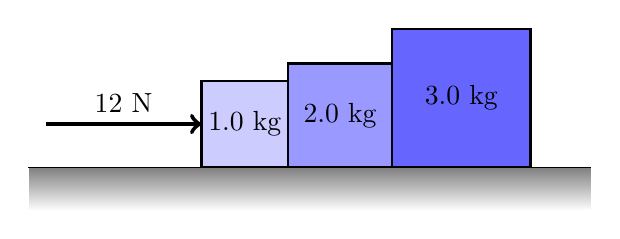
\begin{tikzpicture}[scale=1.1]
      \fill[draw=white,top color=gray,bottom color=white]
      (-2,0)--(4.5,0)--(4.5,-.5)--(-2,-.5)--cycle;
      \draw(-2,0)--(4.5,0);
      \draw[thick,fill=blue!20] rectangle(1,1) node[midway]{1.0 kg};
      \draw[thick,fill=blue!40](1,0) rectangle (2.2,1.2) node[midway]{2.0 kg};
      \draw[thick,fill=blue!60](2.2,0) rectangle (3.8,1.6) node[midway]{3.0 kg};
      \draw[ultra thick,->] (-1.8,.5)--(0,.5) node[midway,above]{12 N};
    \end{tikzpicture}
  \end{center}
  
\item Find the tension in each cord for the systems shown in the figure below
  when it is in static equilibrium (i.e.\ all forces are balanced). The cords
  have negligible mass.
  \begin{center}
    \begin{tikzpicture}
      \fill circle (.05);
      \fill[pattern=north east lines] (-2.5,3)--(-2.5,3.5)--(2.5,3.5)--
      (2.5,-2)--(2,-2)--(2,3)--cycle;
      \draw[thick] (-2.5,3)--(2,3)--(2,-2);
      \begin{scope}[very thick]
        \draw (0,0)--(-2,3) node[midway,left]{$T_1$} node[pos=.9,right]{\ang{60}};
        \draw (0,0)--(2,0) node[midway,below]{$T_2$};
        \draw (0,0)--(0,-1) node[midway,left]{$T_3$};
      \end{scope}
      \shade[ball color=green!70!black] (0,-1.5) circle (.5)
      node[right]{\quad\SI{100}\newton};
    \end{tikzpicture}
  \end{center}
  
\item A curling stone with mass 20.0 kg leaves the curler's hand at a speed of
  \SI{.885}{\metre\per\second}. It slides \SI{31.5}{\metre} down the rink
  before coming to rest. 
  \begin{enumerate}[itemsep=3pt]
  \item Draw a free-body diagram of the curling stone after it leaves the
    curler's hand
  \item Find the average force of friction acting on the stone
  \item Find the coefficient of kinetic friction between the ice and the stone
  \item How far would the curling stone travel if its mass was reduced to
    \SI{15.}{\kilo\gram}, if the initial velocity is the same?
  \end{enumerate}

\item A bike with mass \SI{6.8}{\kilo\gram}, with a cyclist (mass
  \SI{63.5}{\kilo\gram}), are travelling at \SI{45.4}{\kilo\metre\per\hour}
  during a bike race, when the cyclist sees a crash ahead. To avoid the crash,
  he applies the brakes, locking the wheels.
  \begin{enumerate}
  \item How far does the bike travel if the coefficient of kinetic friction
    between the tires and the road is 0.60?
  \item How far would the bike travel if the mass of the cyclist is only
    \SI{40.2}{\kilo\gram}?
  \end{enumerate}
  
\item A skier coasts down a \ang{3.5} slope at constant speed.
  \begin{enumerate}[itemsep=3pt]
  \item Draw a free-body diagram of the skier. The skier should be represented
    by a dot. All forces (not components) should be drawn as arrow that
    originate at, and pointing away from, the dot.
  \item Find the coefficient of kinetic friction between the skis and the snow
    covering the slope.
  \end{enumerate}
  (Hint: If you solve the problem algebraically first, \emph{most} of the
  variables will cancel out, leaving you with a \emph{very} simple expression.
  That's the time to substitute numerical values for your final answer.)
  
%\item A pulley device is used to hurl projectiles from a ramp ($\mu_k=0.26$).
%  Mass A (\SI{5.}{kg}) is accelerated from rest at the bottom of the
%  \SI{4.}{m}-long
%  ramp by mass B, a falling \SI{20.}{kg} mass suspended over a frictionless
%  pulley.
%  Just as A reaches the top of the ramp, it detaches from the rope (neglect the
%  mass of the rope) and becomes projected from the ramp.
%  \begin{enumerate}[noitemsep,topsep=0pt,leftmargin=18pt]
%  \item Draw free-body diagrams for both masses. (Draw forces directly on the
%    diagram.)
%  \item Determine the acceleration of A along the ramp.
%  \item Determine the tension in the rope during the acceleration of A along
%    the ramp.
%  \item Determine the speed of projection of A from the top of the ramp. 
%  \item Determine the horizontal range of A from the base of the ramp.
%  \end{enumerate}
%  \pic{.45}{diagram2}
%  \vspace{2.5in}
  
%\item One method to increase the storage space in a very small house is to
%  hang storage bins from the ceiling using ropes. In this example, a
%  \SI{26}{\kilo\gram} bin is hung from the ceiling using two ropes of different
%  tension, as shown in the diagram below. What is the tension in each of the
%  ropes? (Hint: Start with a free-body diagram at the junction between the
%  ropes.
%  \begin{center}
%    \begin{tikzpicture}[scale=1.2]
%      \draw[mass] (-1,.7) rectangle (1,2) node[midway]{\SI{26}{\kilo\gram}};
%      \draw[ultra thick,brown] (0,2)--(0,2.5);
%      \draw[ultra thick,brown] (3,3.5)--(0,2.5)--(-1.5,3.5);
%      \fill[pattern=north east lines] (-3,3.5) rectangle (4,3.8);
%      \draw[very thick] (-3,3.5)--(4,3.5);
%      \fill (0,2.5) circle (.06);
%      \draw[axes] (2,3.5) arc (180:198.4:1) node[midway,left]{\ang{18.4}};
%      \draw[axes] (-0.5,3.5) arc (0:-33.7:1) node[midway,right]{\ang{33.7}};
%    \end{tikzpicture}
%  \end{center}
%  \vspace{\stretch1}
%  \newpage

\item Two blocks of masses $m=\SI{.80}{\kilo\gram}$ and
  $M=\SI{2.0}{\kilo\gram}$ are connected by a massless string over a massless
  and frictionless pulley as shown in the diagram below. The blocks are
  released from rest at $t=0$.
  \begin{center}
    \begin{tikzpicture}
      \draw[thick,brown] (-3,.4)--(.1,.4);
      \draw[thick] (0,0)--(-5.5,0) node[midway,below]{$\mu=0.14$};
      \draw[mass] (-3,0) rectangle +(-1,.8) node[midway]{$m$};
      \begin{scope}[rotate=-30]
        \draw[thick,brown] (1,.4)--(-.05,.4);
        \draw[thick] (0,0)--(4.5,0)
        node[midway,below,rotate=-30] {$\mu=0.14$};
        \draw[thick,mass] (1,0) rectangle +(2,1) node[midway,rotate=-30]{$M$};
      \end{scope}
      \begin{scope}[rotate=-15]
        \draw[thick,fill=gray] (0,.3) circle (.15);
        \draw[thick,fill=gray!50] (0,.3) circle (.1);
        \draw[ultra thick] (0,0)--(0,.3);
        \fill (0,.3) circle (.04);
      \end{scope}
      \draw[thick,gray!70] (0,0)--(0,-1.5);
      \draw[axes] (0,-.5) arc (270:330:.5)
      node[midway,below]{$\phi=\ang{60}$};
    \end{tikzpicture}
  \end{center}
  \begin{enumerate}
  \item Draw free-body diagrams of the blocks as they move.
  \item Determine the magnitude of acceleration of the blocks.
  \item Calculate the magnitude of the tension force in the string.
      %\item If the string broke, for what minimum value of the coefficient of
      %static friction would the \SI{2.0}{\kilo\gram} block not begin to slide?
  \end{enumerate}
%    (Some hints and FYI: The pulley \emph{must} be frictionless and massless,
%    otherwise, when the blocks are released from rest, the pulley will have
%    rotational kinetic energy, and the tension will not be constant throughout.
%    Both blocks will have the same magnitude of acceleration. To solve the
%    problem, apply the second law of motion to each block, and the two unknowns
%    that you need to solve are acceleration an tension. It does not matter which
%    quantity you solve first.)
    
\item In the figure below, the blocks do not slide against each other when
  horizontal external force $\bm F$ is applied to $m_3$, as shown in the
  figure below. Assume that there is no friction at the contact between the
  blocks and the table. (Note: Without this external force $\bm F$, $m_2$
  would accelerate downwards, while $m_1$ would accelerate towards the right.)
  \begin{center}
    \begin{tikzpicture}[scale=1.1]
      \draw[very thick] (-3,0)--(3,0);
      \fill[pattern=north east lines] (-3,0) rectangle (3,-.3);
      \begin{scope}[thick]
        \draw[mass] (-1.7,0) rectangle (0,1.2) node[midway]{$m_3$};
        \draw[fill=gray!70] (-1.7,1.2) rectangle (-.8,1.9)
        node[midway]{$m_1$};
        \draw[fill=gray!70] (0,.3) rectangle (.6,.78) node[midway]{$m_2$};
      \end{scope}
      \begin{scope}[ultra thick,brown]
        \draw (-.8,1.55)--(.1,1.55);
        \draw (.35,1.2)--(.35,.78);
      \end{scope}
      \begin{scope}[very thick]
        \draw[fill=lightgray] (.1,1.3) circle (.3);
        \draw[fill=gray] (.1,1.3) circle (.2);
      \end{scope}
      \fill (.1,1.3) circle (.05);
      \draw[vectors] (-2.6,.6)--(-1.7,.6) node[pos=0,left]{$\bm F$};
    \end{tikzpicture}
    
    $m_1=\SI{1.8}{\kilo\gram}$, $m_2=\SI{1.2}{\kilo\gram}$,
    $m_3=\SI{3.0}{\kilo\gram}$
  \end{center}    
  \begin{enumerate}[itemsep=3pt]
  \item Draw free-body diagrams for each of the blocks. The block should be
    presented by a dot. Forces should be drawn as arrows originating at, and
    pointing away from, the dot that represent the object.
      
    %\uplevel{
    %  Hints: For parts (b) and (c), you will only need to use the free-body
    %  diagrams of two of the 3 blocks. If the blocks don't slide against each
    %  other, they will all have the same acceleration vector.)
    %}
  \item Calculate the acceleration of the blocks (both magnitude and
    direction) when the force is applied.
  \item Calculate the magnitude of the force applied
  \end{enumerate}
    
\item In a tractor-pull competition, a tractor applies a force of
  \SI{1.3}{\kilo\newton} to the sled, which has mass \SI{1.1e4}{\kilo\gram}. At
  that point, the coefficient of kinetic friction between the sled and the
  ground has increased to 0.80. What is the acceleration of the sled? Explain
  the significance of the sign of the acceleration. 
 
\item A solo Arctic adventurer pulls a string of two toboggans of supplies
  across level, snowy ground. The toboggans have masses of \SI{95}{\kilo\gram}
  and \SI{55}{\kilo\gram}. Applying a force of \SI{165}{\newton} causes the
  toboggans to accelerate at \SI{.61}{\metre\per\second\squared}.
  \begin{enumerate}[itemsep=3pt]
  \item Calculate the frictional force acting on the toboggans. 
  \item Find the tension in the rope attached to the second
    (\SI{55}{\kilo\gram}) toboggan.
  \end{enumerate}

%  \item A \SI{3.0}{\kilo\gram} counterweight is connected to a
%  \SI{4.5}{\kilo\gram} window that freely slides vertically in its frame. How
%  much force must you exert to start the window opening with an acceleration of
%  \SI{.25}{\meter\per\second\squared}.
%  \vspace{\stretch1}
%  \newpage
%
%  %\uplevel{
%  %  \pic{.35}{../graphics/pulley-a-b}
%  %}
%  %\item A rope of negligible mass passes over a pulley of negligible
%  %mass attached to the ceiling, as shown above. One end of the rope is held by
%  %Student $A$ of mass \SI{70}{\kilo\gram}, who is at rest on the floor. The
%  %opposite end of the rope is held by Student $B$ of mass \SI{60}{\kilo\gram},
%  %who is suspended at rest above the floor.
%  %\begin{enumerate}[itemsep=3pt]
%  %  \item On the dots below that represent the students, draw and label
%  %  free-body diagrams showing the forces on Student $A$ and on Student $B$.
%  %
%  %  \vspace{.3in}
%  %  \begin{center}
%  %    \begin{tikzpicture}
%  %      \fill circle (.08) node[right]{$\;A$};
%  %      \fill (1,2.5) circle (.08) node[right]{$\;B$};
%  %    \end{tikzpicture}
%  %  \end{center}
%  %  \vspace{.3in}
%  %  
%  %  \item Calculate the magnitude of the force exerted by the floor on Student
%  %  $A$.
%  %  
%  %  \uplevel{
%  %    Student $B$ now climbs up the rope at a constant acceleration of
%  %    \SI{.25}{\metre\per\second\squared} with respect to the floor.
%  %  }
%  %  
%  %  \item Calculate the tension in the rope while Student B is accelerating.
%  %
%  %  \item As Student $B$ is accelerating, is Student $A$ pulled upward off the
%  %  floor? Justify your answer.
%  %
%  %  \item With what minimum acceleration must Student $B$ climb up the rope to
%  %  lift Student $A$ upward off the floor?  
    %  %\end{enumerate}

\item A small block of mass $m=\SI{2.0}{\kilo\gram}$ sits on a larger block of
  mass $M=\SI{4.0}{\kilo\gram}$ that is resting on a table, as shown below. The
  bottom block is being pulled to the right by an external force $\bm F$.
  \begin{center}
    \begin{tikzpicture}[scale=1.4]
      \draw[thick] (-1,0)--(4,0);
      \draw[thick,fill=gray!70] rectangle (2,1) node[midway]{$M$};
      \draw[thick,fill=gray!40] (.5,1) rectangle (1.5,1.75) node[midway]{$m$};
      \draw[vectors] (2,.5)--(3.5,.5) node[right]{$\bm F$};
    \end{tikzpicture}
  \end{center}
  The coefficients of static and kinetic friction between the blocks are
  $\mu_s=0.30$ and $\mu_k=0.20$, respectively. There is no friction between
  $M$ and the table.
  \begin{enumerate}[itemsep=3pt]
  \item In a clearly labelled free-body diagram, draw and label all
    forces (not components) acting on the blocks. Forces should be drawn as
    arrow beginning, and pointing away from, the dots that represent the
    blocks.
      
  \item What is the maximum acceleration that the blocks can have without
    $m$ sliding against $M$?
    
  \item What is the maximum force $\bm F$ that can be applied if the
    \SI{2.0}{\kilo\gram} block is not to slide on the \SI{4.0}{\kilo\gram}
    block.\label{partA}
    
  \item If $\bm F$ is half the value found in (\ref{partA}), find the
    acceleration of each block and the force of friction acting on each block.
    
  \item If $\bm F$ is twice the value found in (\ref{partA}), find the
    acceleration of each block.
  \end{enumerate}
  \begin{center}
    \begin{tikzpicture}
      \fill[pattern=north east lines] rectangle (5,-.3);
      \draw[thick] (0,0)--(5,0);
      \draw[thick,fill=gray!70] (1,0) rectangle (4,1.5) node[midway]{100 kg};
      \draw[thick,fill=gray!20] (1,1.5) rectangle (2.5,2.5) node[midway]{60 kg};
      \draw[vectors] (2.5,2)--(3.8,2) node[right]{$\bm F$};
    \end{tikzpicture}
  \end{center}

\item A \SI{60}{\kilo\gram} block slides along the top of a
  \SI{100}{\kilo\gram} block with an acceleration of
  \SI{3.0}{\metre\per\second\squared} when a horizontal force of
  $F=\SI{320}\newton$ is applied, as shown in the figure above. The 
  \SI{100}{\kilo\gram} block sits on a horizontal frictionless table, but there
  is friction between the two blocks.
  \begin{enumerate}
  \item In clearly labelled free-body diagrams, draw and label all forces (not
    components) acting on the blocks. Forces should be drawn as arrow
    orginating at, and pointing away from, the dots that represent the blocks.

  \item Find the coefficient of kinetic friction between the blocks.
    
  \item Find the acceleration of the \SI{100}{\kilo\gram} block during the
    time that the \SI{60}{\kilo\gram} block maintains contact.
  \end{enumerate}
  \begin{center}
    \begin{tikzpicture}[scale=2.1]
      \draw[vectors] (.5,.6)--(1.7,.6) node[right,black]{$\bm a$};
      \draw[thick] (-1,0)--(2,0);
      \draw[thick,fill=lightgray] (0,0)--(0,1.7)--(1,0)--cycle;
      \draw[axes] (.7,0) arc (180:120:.3) node[midway,left]{\ang{60}};
      \begin{scope}[rotate around={-59.5:(1,0)}]
        \draw[thick,fill=gray!70] rectangle (-.5,.5)
        node[midway]{\SI{2.0}{\kilo\gram}};
      \end{scope}
    \end{tikzpicture}
  \end{center}

\item A \SI{2.0}{\kilo\gram} body rests on a smooth wedge that has an
  inclination of \ang{60} and an acceleration $\bm a$ to the right such that
  the mass remains stationary relative to the wedge.
  \begin{enumerate}
  \item Find acceleration $\bm a$.
  \item What would happen if the wedge were given a greater acceleration?
  \end{enumerate}
  
\item A pick-up truck with two stacked crates in the truck bed brakes
  quickly. The crate on the bottom just barely stays put on the bed of the
  truck. Does the top crate stay put or does it fall off? The top crate has a
  mass of \SI{27}{\kilo\gram} and the mass of the bottom crate is
  \SI{22}{\kilo\gram}. The coefficient of static friction between the bottom
  crate and the truck is 0.42, and the coefficient of kinetic friction for
  that surface is 0.35. The coefficient of static friction between the crate
  is 0.40, and the coefficient of kinetic friction is 0.32.  
  \begin{center}
    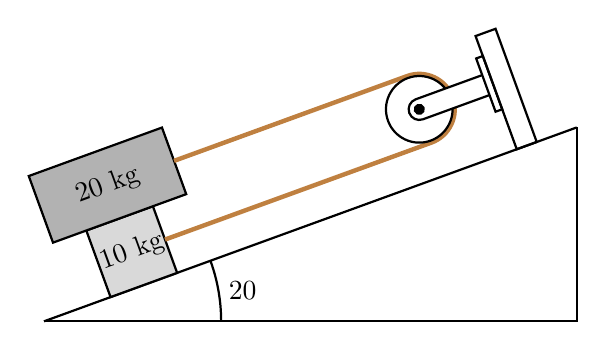
\begin{tikzpicture}[scale=.9]
      \begin{scope}[rotate=20,thick]
        \draw (0,0)--(8,0);
        \draw[fill=gray!30] (1,0) rectangle (2,1)
        node[midway,rotate=20]{10 kg};
        \draw[fill=gray!60] (.5,1) rectangle (2.5,2)
        node[midway,rotate=20]{20 kg};
        \draw[ultra thick,brown] (2,.5)--(6,.5) arc (-90:90:.5)--(2.5,1.5);
        \draw (6,1) circle (.47);
        \draw[fill=white] (7,.85)--(6,.85) arc (270:90:.15)--(7,1.15);
        \draw (7.1,0) rectangle (7.4,1.7);
        \draw (7,.6) rectangle (7.1,1.4);
        \fill (6,1) circle (.08);
      \end{scope}
      \draw[thick] (0,0)--(8*cos{20},0)--(8*cos{20},8*sin{20});
      \draw[thick] (2.5,0) arc (0:20:2.5) node[midway,right]{\ang{20}};
    \end{tikzpicture}
  \end{center}

\item The figure above shows a \SI{20}{\kilo\gram} block sliding on a
  \SI{10}{\kilo\gram} block. All surfaces are frictionless.
  \begin{enumerate}
  \item The dots below represent the blocks. Draw and label all forces (not
    components) acting on the blocks. Forces should be drawn as arrow
    orginating at, and pointing away from, the dots.
%      \uplevel{
%        \centering
%        \vspace{.8in}
%        \begin{tikzpicture}
%          \fill circle (.15) node[left=3]{20 kg};
%          \fill (5,0) circle (.15) node[right=3]{10 kg};
%      \end{tikzpicture}
%        \vspace{.8in}
%    }
  \item Find the acceleration of each block    
  \item Find the tension that connects the blocks.
  \end{enumerate}
\end{enumerate}

